\section{Exploración Dimensión del Cromosoma}

\begin{table}[]
    \centering
    \begin{tabular}{||c|c|c|c|c|c||}
        \hline
        \textbf{Fichero Configuración} & \textbf{Generaciones} & \textbf{DIM} & \textbf{Tmñ. poblacion} & \textbf{Mejor fitness} & \textbf{Evals. de f}\\ \hline
        Config 10  & 45   & 10    & 1000   & -38.48    &  69537    \\ \hline
        Config 11  & 92   & 15    & 1500   & -38.88    &  211163   \\ \hline
        Config 12  & 62   & 30    & 3000   & 79.74     &  288787   \\ \hline
        Config 13  & 78   & 50    & 5000   & 346.941   &  602536   \\ \hline
        Config 14  & 94   & 100   & 10000  & 1266.01   &  1459146  \\ \hline
    \end{tabular}
    \caption{Resultados exploración inicial}
    \label{tab:exploracion_dim_cromosoma}
\end{table}

Para realizar esta exploración se ha seguido el mismo proceso que en las anteriores. El algoritmo se ha ejecutado 15 veces por cada fichero de configuración.
Se toma como base el tamaño de población 1000, que irá variando proporcionalmente a la dimensión del cromosoma. El resumen de estas ejecuciones está en la 
Tabla \ref{tab:exploracion_dim_cromosoma}. 

\begin{figure}[]
	\centering	
	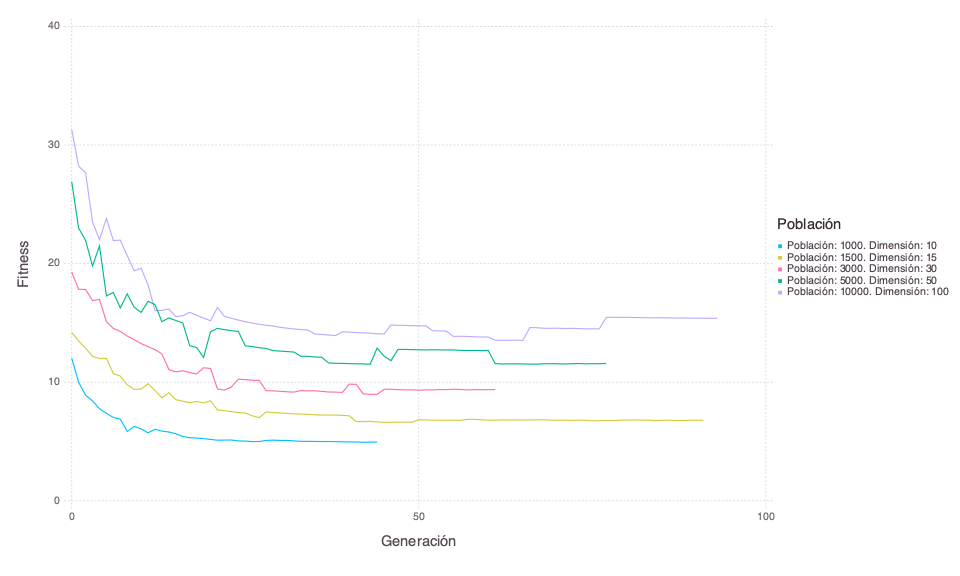
\includegraphics[scale=0.5]{figuras/ps_cd_variation.png}
	\caption{ Variación del fitness a lo largo de las generaciones }
    \label{fig:exec_summary}
\end{figure}

\begin{figure}[]
	\centering	
	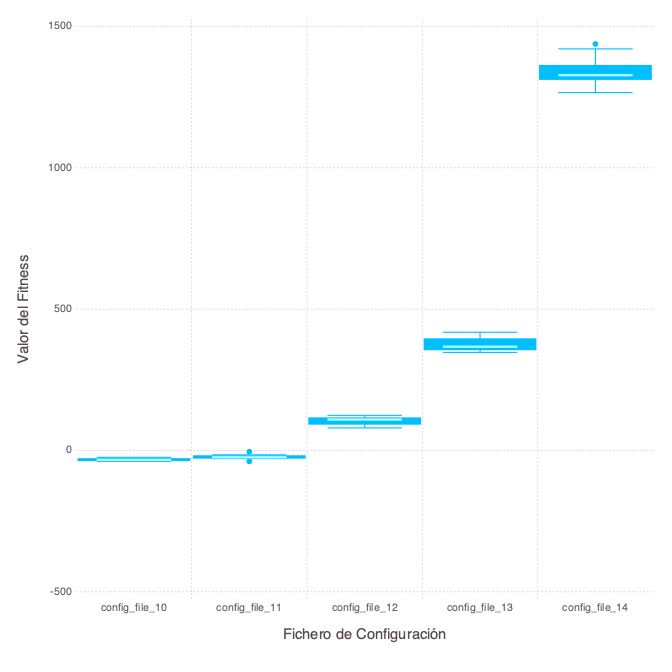
\includegraphics[scale=0.5]{figuras/Rastrigin_box_plots_chrom_dim.png}
	\caption{ Variación de los resultados, variando la dimensión del cromosoma }
    \label{fig:box_plots_crom_dim}
\end{figure}

Viendo la Figura \ref{fig:exec_summary}, todas las ejecuciones tienen un comportamiento parecido, gran descenso del valor del fitness al principio. Además,
en la Figura \ref{fig:box_plots_crom_dim} como, exceptuando las dos primeras configuraciones, cada una tiene un espacio de búsqueda diferente. Una conclusión
que podemos sacar de esta figura es que la exploración del espacio no es muy exhaustiva, al contrario que la explotación, que queda reflejada en el número de ejecuciones
de la función de fitness. En las siguientes exploraciones se tratará de cambiar el ratio de mutación para intentar aumentar la exploración del algoritmo. 
Además se usará 50 como dimensión del cromosoma, siguiendo como criterio el valor del fitness y la exploración que realiza, la configuración 13 es la ganadora.